\section{Coloraci\'on m\'as all\'a de los tableros}

Es un hecho de que colorear tableros es bastante \'util. Sin embargo, coloraciones en otras situaciones tambi\'en pueden ser bastante \'utiles. Es cuesti\'on de reconocer cu\'ando la situaci\'on es id\'onea para la coloraci\'on e intentarlo. Desde luego, como ya no se tratan de tableros en esta vuelta, nuestra amada receta deber\'a ser adaptada o descartada en todo caso.

\subsection{Problemas}

\begin{enumerate}
	\item Pruebe que dados $n>5$ puntos en el plano, de los cuales no hay tres colineales, es posible colorearlos de dos colores de manera que no exista una linea que separe los puntos de un color a los puntos del otro color (la l\'inea no puede pasar por ningun punto).
	
	\item Se tiene un c\'irculo dividido en $6$ sectores iguales y se escriben los n\'umeros 1, 0 1, 0, 0, 0, uno en cada secci\'on de manera ordenada. Si un movimiento consiste en sumar o restar $1$ a dos secciones adyacentes, ¿Se puede llegar, despu\'es de una cantidad finita de movimientos, a tener todas las secciones del c\'irculo con un  mismo n\'umero?.
	
	\item Se tiene un pa\'is con ciudaddes conectadas como en la figura siguiente:
	\begin{center}
		\begin{figure}[h!]
			\centering
			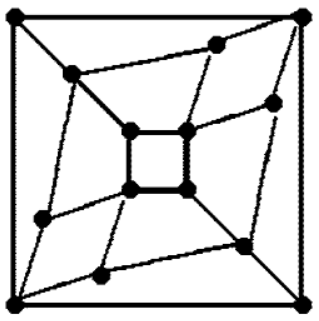
\includegraphics[scale=.5]{imgs/cities.png}
		\end{figure}
	\end{center}
	Deterimne si es posible visitar todas las ciudades exactamente una vez.
	
	\item Pruebe que es imposible dibujar un camino con el l\'apiz de maera que intersecte a todos los segmentos de la figura exactamente una vez (y no se est\'a permitido pasar por las esquinas).
	\begin{center}
		\begin{figure}[h!]
			\centering
			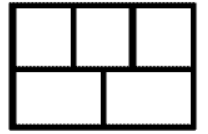
\includegraphics[scale=.4]{imgs/curve.png}
		\end{figure}
	\end{center}
	
	\item Cada punto del plano se pinta de rojo o azul. Demuestre que existen tres puntos del mismo color, de modo que uno de los puntos es el punto medio del segmento formado por los otros dos puntos
	
	\item Determine si es posible pintar cada uno de los enteros de rojo, azul o verde, de manera que se cumplan las siguientes condiciones:
	\begin{enumerate}[a.]
		\item Existe al menos un n\'umero de cada color.
		\item Si $ a+b = c$, y $a$ y $b$ son de colores diferentes, entonces $c$ es de color rojo.
	\end{enumerate}
	
	\item Se pintan los enteros positivos de negro o blanco, de manera que la suma de dos n\'umeros de diferentes colores es blanca y el producto es negro. 
\end{enumerate}